\chapter{Readout Infidelity Budget} \label{chap:budget}
With a simulation realistically representing the qubit-resonator system from the laboratory, we are now in a position to break down the different effects on the readout fidelity. In this section, we will leverage the simulation tools, to quantify the contributions to the infidelity from the different physical processes, we have included in our model. Thereafter, we will try to break down, how different improvements of the physical parameters will have an effect on the fidelity of our readout. 
\section{Turning off the Contributions}
In this section, we will hypothesize three contributions to our SPAM fidelity. By then turning on and off the different elements from here, we will try to quantize the effect they have on the errors of our readout procedure. The three hypothesis are.
\begin{enumerate}
    \item A low readout efficiency, $\eta$, results in overlap between the $\ket{0}$ and $\ket{1}$ distributions in the IQ plane. The results in a readout assignment error 
    \item The temperature, $\tau$, is contributing significantly to the initialization error. At non-zero temperature, we will expect to see a mixed state with non-zero elements for $\ket{1}\bra{1}$. These errors will not be detected during readout. 
    \item Energy exchanges with the environment can give a low coherence time $T_1$. Since relaxation or excitation during the readout will make the system behave like it is in the other state, this will lead to wrong classifications.
\end{enumerate}
By using the model which we built up in chapter \ref{chap:model}, we can now turn off the different contributions and see the resulting fidelity of the readout sequence. As a start, we will model the perfect system. That is a system where the qubit has infinite lifetime $T_1 = \infty$, the system will be zero temperature, $\tau = 0$ and we detect all of the signal $\eta = 1$. A comparison of the Fidelity of this perfect system and the realistic one, which we also simulated in section \ref{sec:readout_in_simulation} can be seen in table \ref{tab:realistic_perfect_comparison} and the corresponding IQ plot is found in figure \ref{fig:realistic_perfect_comparison}. To see weights, histograms and other details, we refer to appendix \ref{chap:IQ_plots}.


\begin{figure}
    \centering
    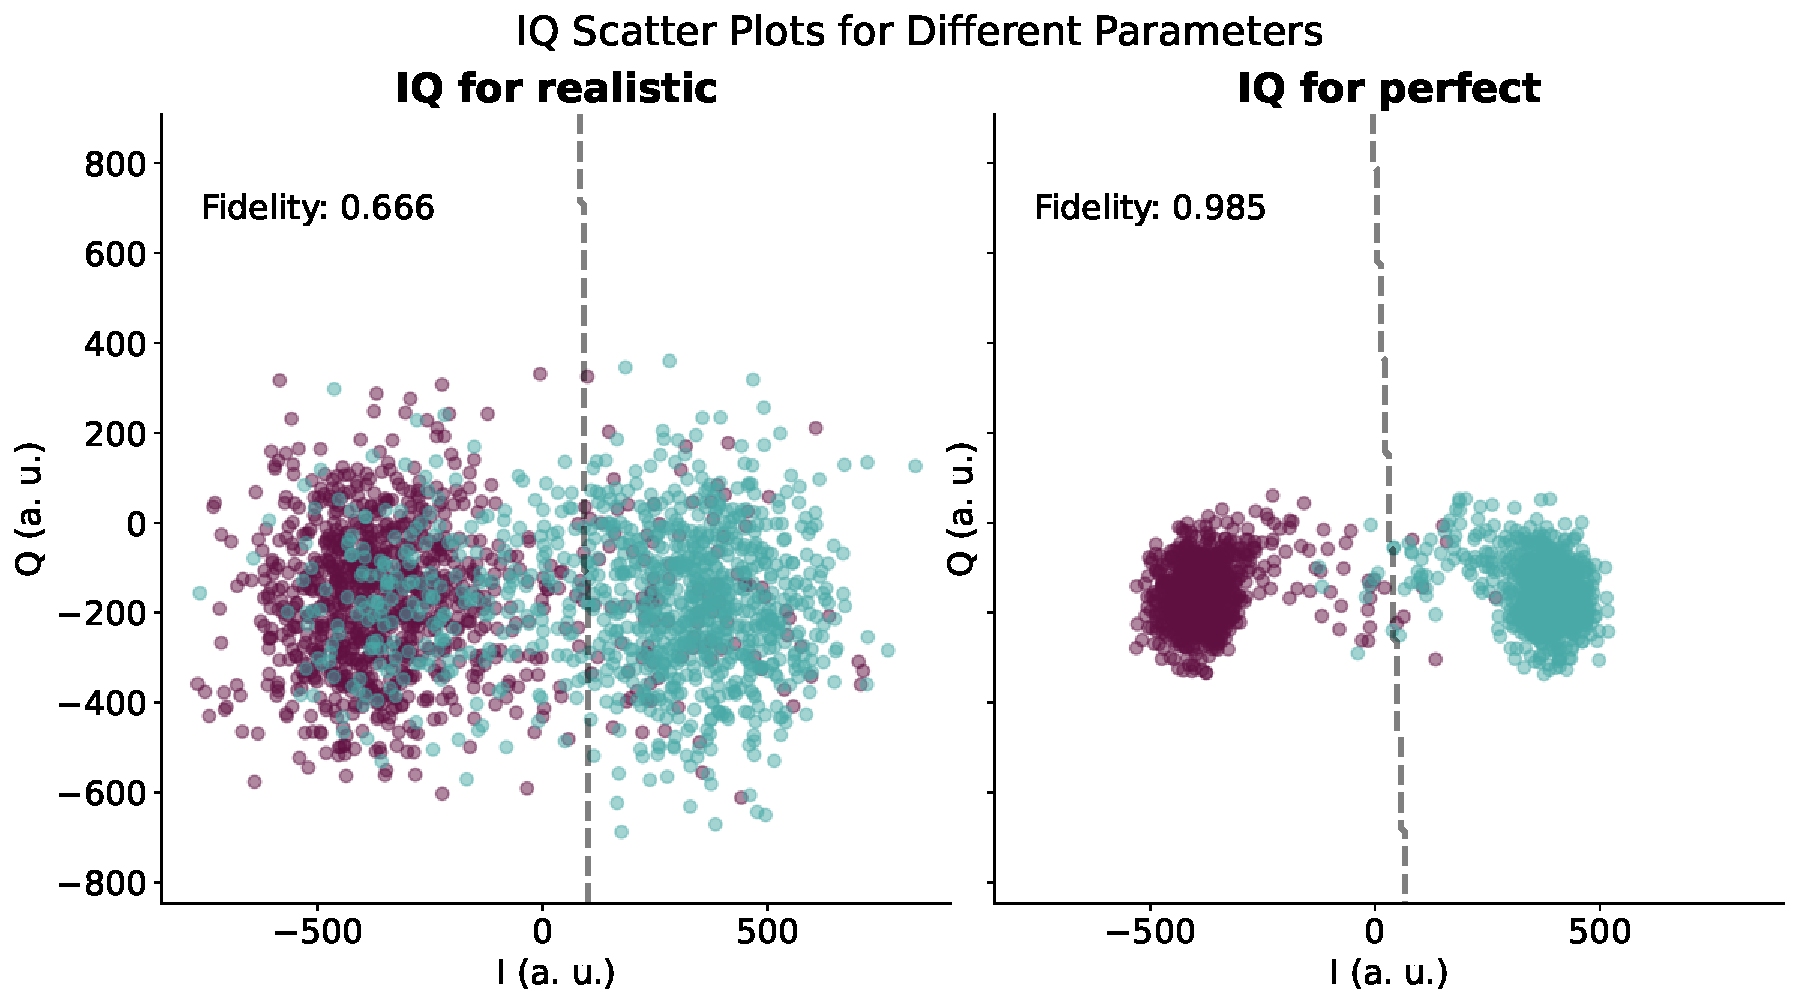
\includegraphics[]{Simulations/budgets/figures/iq_scatter_budgetting_on_off_two.pdf}
    % \missingfigure[figheight = \textheight / 3]{IQ Plots for the simulation, we ran in the table}
    \caption{The IQ distributions for the experiment run with a realistic and an ideal set of parameters. The fidelity as well as separation line is shown on the plot. }
    \label{fig:realistic_perfect_comparison}
\end{figure}

\begin{margintable}[-2 cm]
    \centering
    \caption{Results from running the simulation experiment for 500 samples with a realistic set of parameters and a perfect set of parameters.}
    \begin{tabular}{l|r}
    \hline
         Parameters Set & Fidelity \\ \hline
         Realistic & 0.654 $\pm$ 0.024  \\
         Perfect   & 1.000 $\pm$ 0.000  
    \end{tabular}
    \label{tab:realistic_perfect_comparison}
\end{margintable}
In a model with the perfect parameters, we get fidelity of $F_{\text{SPAM}} = 1$. There are a few points in the middle which is suspected to be the effect we described in section \ref{sec:hilbert_space}, where  the SME in a finite Hilbert Space produces some unwanted dynamics with high efficiency\footnote{The suspicion comes from seeing many more of these points with a lower dimensional Hilbert Space}. If we ignore these points, the hypothesis holds its own when tested in our model. If we eliminate all three elements, we experience no SPAM errors.


In an attempt to single out the effect on readout fidelity from the individual contributions, we can repeat the experiment with the different combinations of turning the effects on one after another. This leads to six experiments. Starting from the realistic set of parameters, we have three experiments with $\eta = 1$, $T_1 = \infty$, $\tau = 0$ respectively (each which excludes one source of SPAM errors). This is repeated with two out of three of the perfect parameters such that we exclusively have one source of SPAM errors. The IQ plots can be seen in figure \ref{fig:on_off_IQ_scatter_combinations} and the associated fidelity scores in table \ref{tab:readout_infidelity_contribution_estimation}.
\begin{figure}[h]
    \centering
    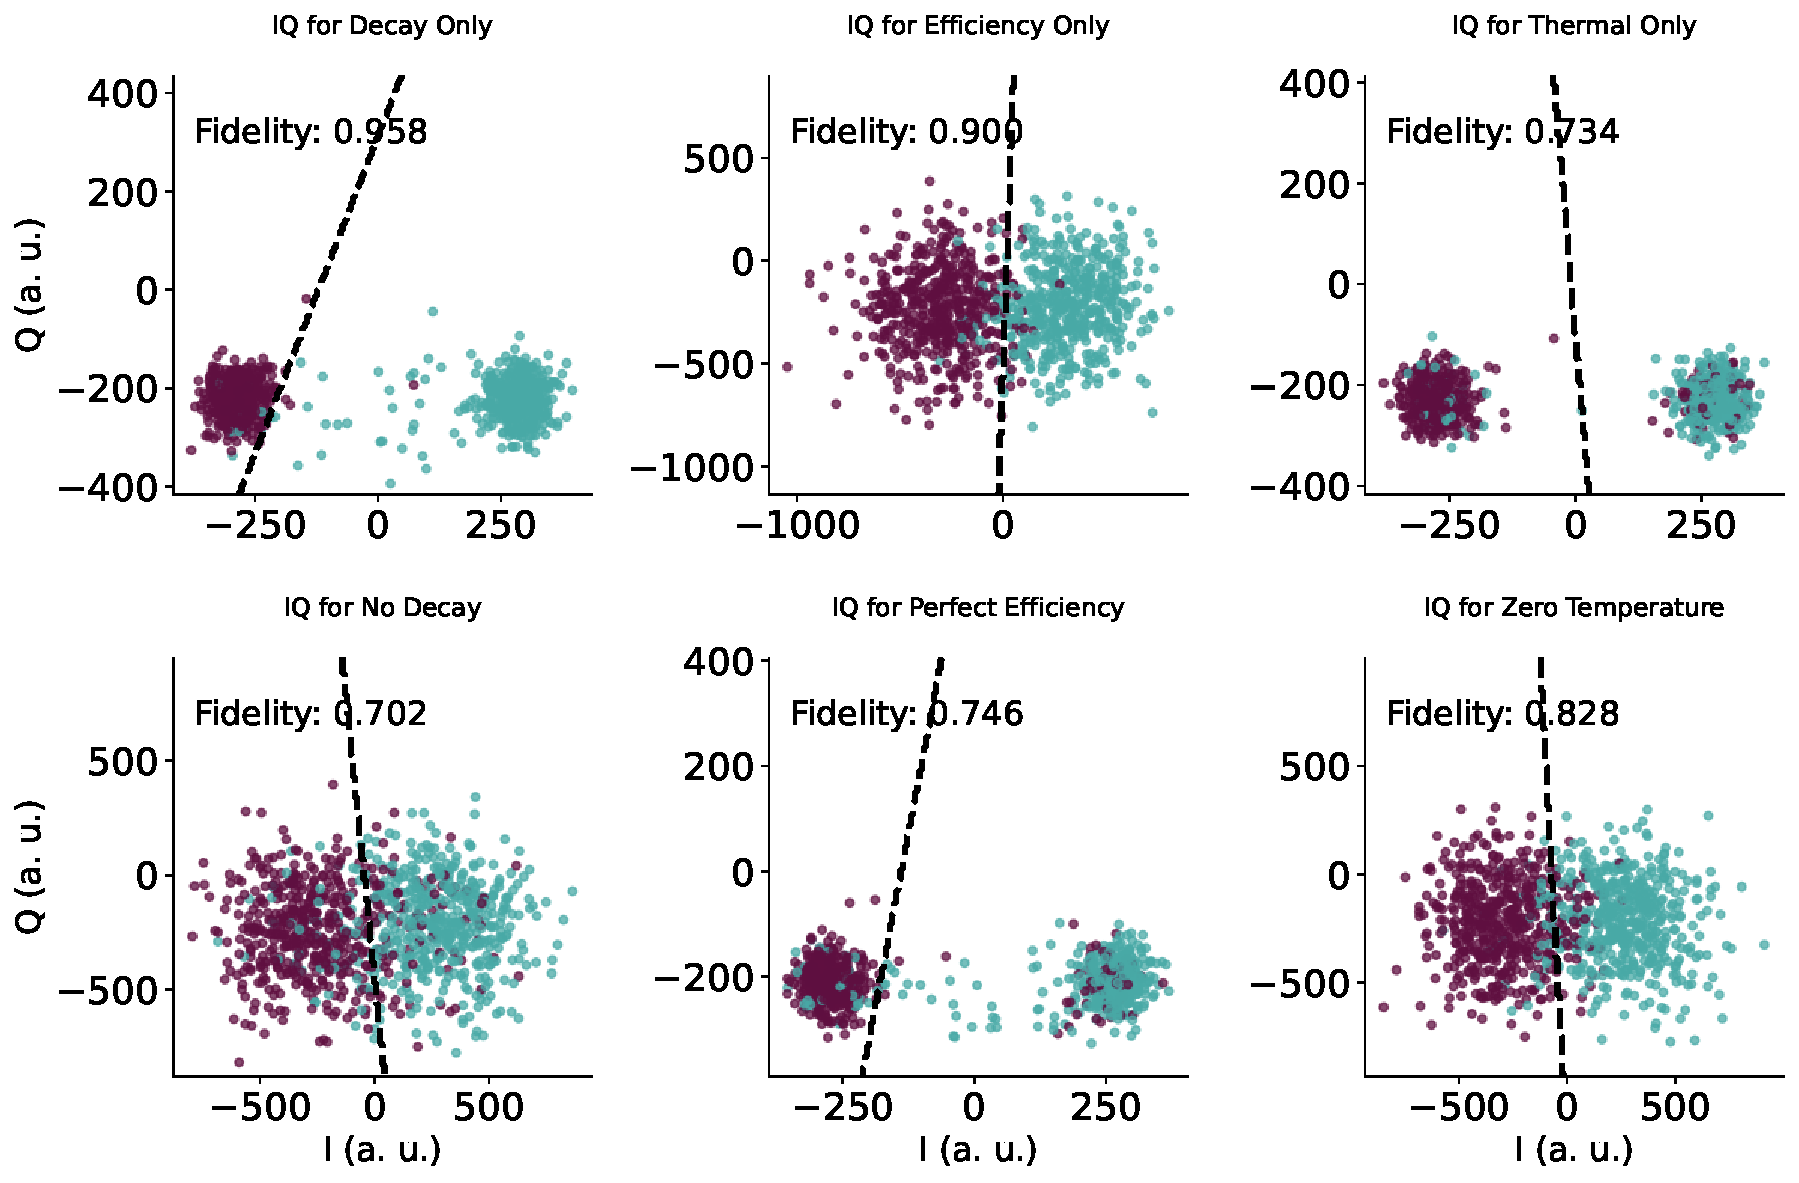
\includegraphics[]{Simulations/budgets/figures/iq_scatter_budgetting_on_off.pdf}
    % \missingfigure[figheight = \textheight / 3]{IQ Plots for the simulation, we ran in the table}
    \caption{The IQ results from turning on the different sources of errors one by one. The IQ scatter plots are displayed along side the decision boundary and the readout fidelity.}
    \label{fig:on_off_IQ_scatter_combinations}
\end{figure}
\begin{table}[h]
\centering
\caption{The Fidelity results of running the simulation experiment with 1000 samples given parameters that sets one or two of the three parameters to the ideal setting.}
\begin{tabular}{l|rrr}
\hline
\textbf{Contributions}        & Temperature         & Energy Decay   & Efficiency  \\ \hline
Excluding                     &  0.828 $\pm$ 0.018  &  0.702 $\pm$  0.022  &  0.746 $\pm$ 0.021\\
Exclusively                   &  0.734 $\pm$ 0.021  &  0.958 $\pm$  0.009  &  0.900 $\pm$ 0.014
\end{tabular}
\vspace{0.3 cm}
\label{tab:readout_infidelity_contribution_estimation}
\end{table}

Another way of visualizing these parameters are by having them in a combination tree and adding one contribution at a time according to the possible permutations. Each time we add a new source of errors we find the increase in infidelity. This will allow us to get a good idea of the contribution from the individual sources. This is done in figure \ref{fig:combination_tree_budget}. With infidelity errors of around $2-3\%$ the differences have errors of $3-4 \%$, so we should be careful extracting too much meaning from the values. We can, however, analyse the overall pattern. At a first glance, the errors does not seem to be additive. Decay adds 7.2 \% infidelity if we have inefficient measurements while the infidelity goes down if we have non-zero temperature. While this could be a 2 sigma outlier, we should be careful when separating the contributions as it looks like there are some second order effects at play as well. If we want to get a vague first order estimate, we take the simple average over infidelity contributions for the different parameters in the combination tree. These averages are shown in table \ref{tab:average_combination_tree}. 
\begin{margintable}[-4 cm]
    \centering
    \caption{Average contribution to infidelity when counting in the combination tree seen in figure \ref{fig:combination_tree_budget}}
    \vspace{0.3 cm}
    \begin{tabular}{l|r}
    \hline
    Parameter       &  Avg Infidelity\\ \hline
    Temperature     & 0.21 \\
    Decay           & 0.04 \\
    Efficiency      & 0.09 \\
    \end{tabular}
    \label{tab:average_combination_tree}
\end{margintable}
\begin{figure*}
    \centering
    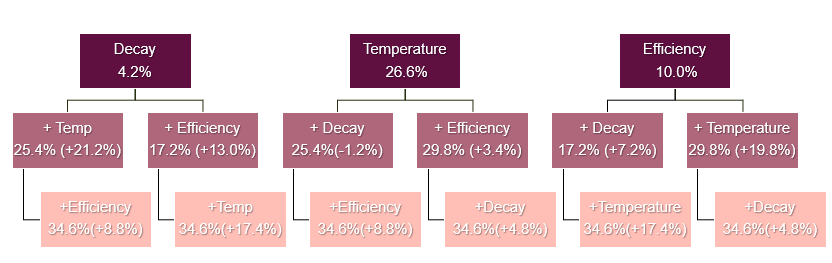
\includegraphics{Figs/Results/combination_tree.png}
    \caption{Visualizing the different ways of combining the error sources and watching their contributions at each step.}
    \label{fig:combination_tree_budget}
\end{figure*}
For our system with a readout pulse defined in section $\ref{sec:overview_section}$, the $F_{\text{SPAM}}$ seems to be dominated by the temperature, followed by inefficiency and lastly the energy decay to the environment. As we will discuss in the next section, there exists multiple tradeoffs which one can use to trade a good parameter for performance corresponding to another.




\section{Improving the Readout}
In this section, we will setup a use case for the developed model. Given the device and the readout pulse parameters used throughout the thesis, what increase in $F_{\text{SPAM}}$ can we the expect by improving the physical device. In context of these improvements, we will discuss how the parameters can be used to improve the performance in other parts of the readout sequence by applying other teckniques. 



% In the previous section, we gave some estimates on how much three different sources contributed to the infidelity in the readout and initialization process. Although these numbers are interesting, an ideal qubit with infinite lifetime or a cooling system capable off sub mini kelvin temperatures are not realistic and is probably not what one should strive for. Instead, we will in this section present more marginal improvements like what would happen if the temperature is reduced by 10\% or 25\%. Furthermore, we will cover some strategies which can be implemented to deal with some of the errors in the straightforward 1 µs readout pulse which we have considered until now.

\subsection{Modifying the Parameters}
\begin{figure*}[t]
    \centering
    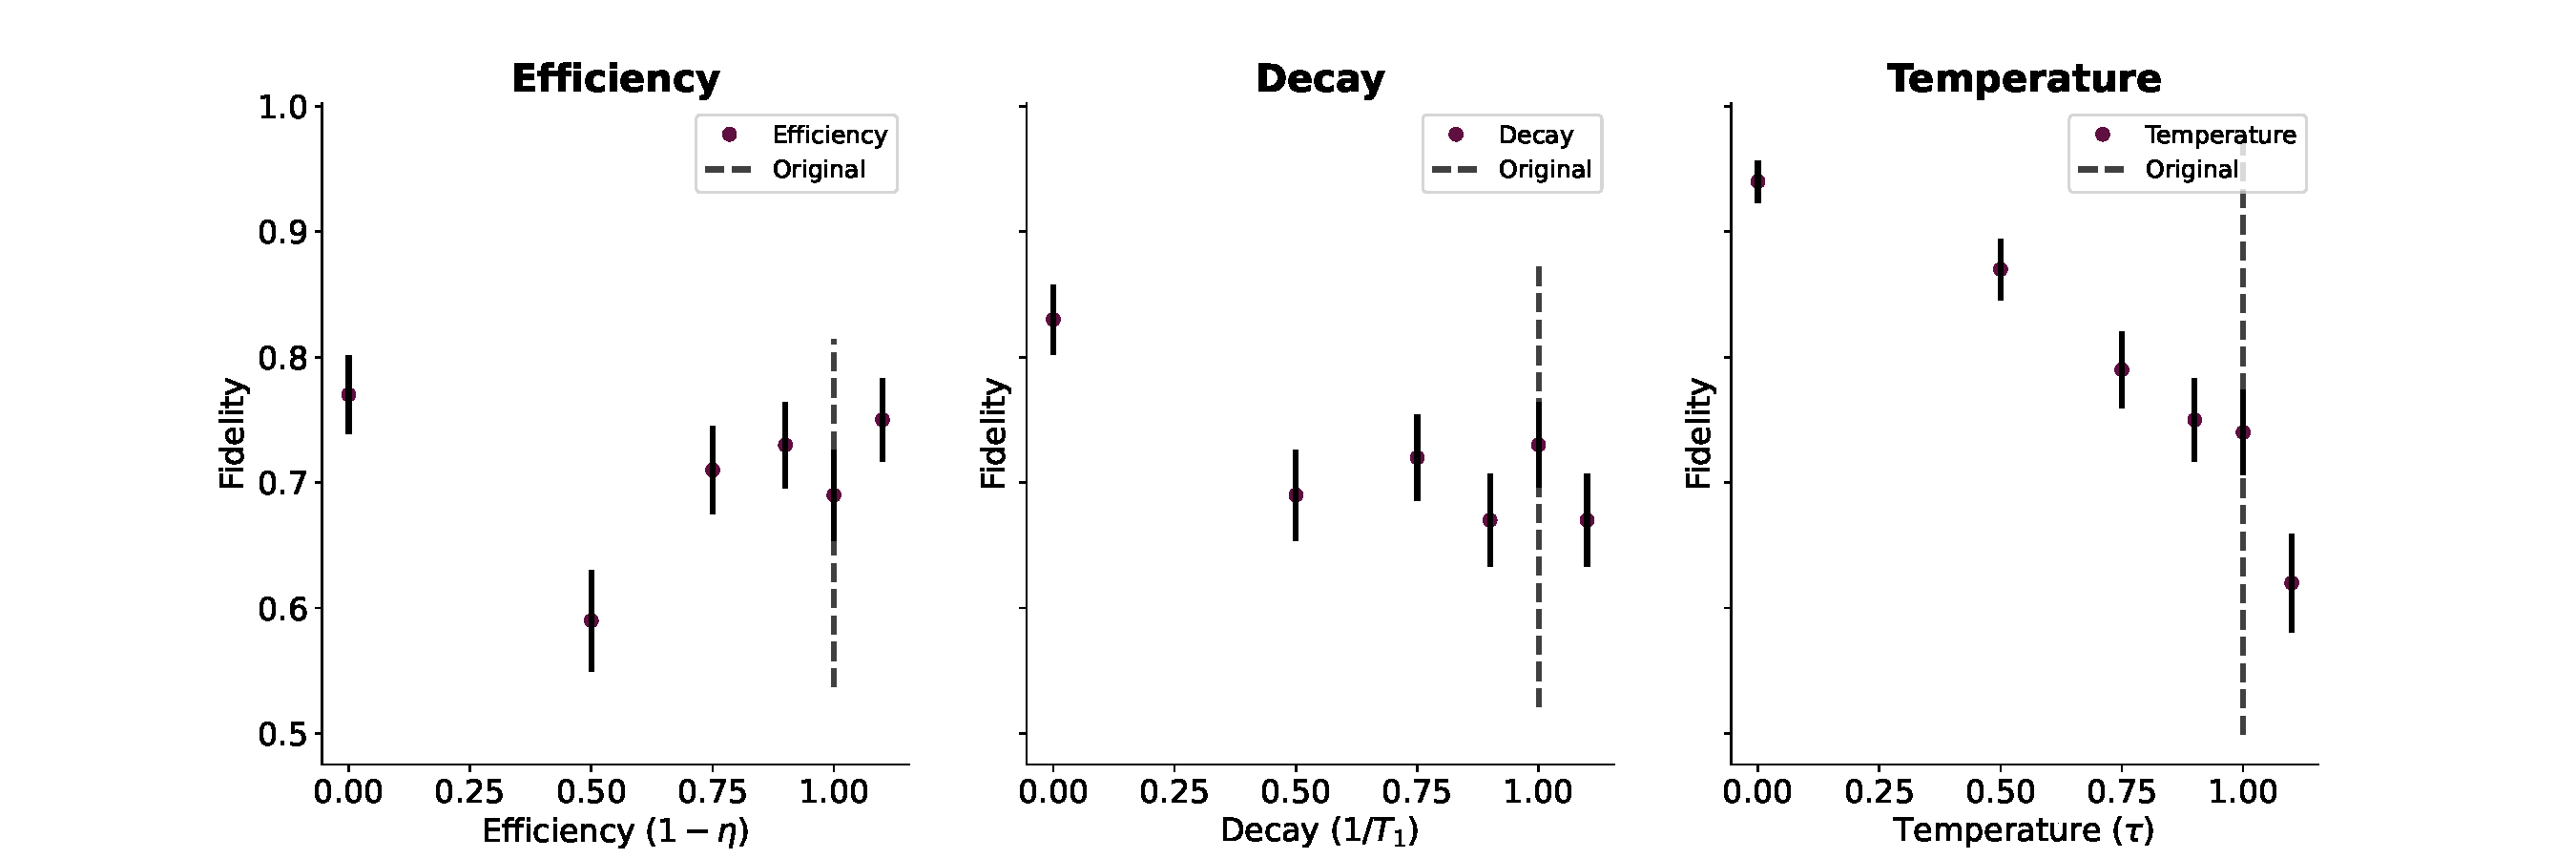
\includegraphics[width = \linewidth]{Simulations/budgets/figures/fidelities_at_different_parameters.pdf}
    \caption{The Fidelities of the model when the parameters are changed. In each plot the two other parameters are held constant at the realistic value.}
    \label{fig:scan_of_fidelities_at_different_parameters}
\end{figure*}
In the previous section, we considered the parameters to be on (at $0$) or off (at $100 \%$) of the considered value. We will now due more incremental improvements of one parameter while we keep the other two fixed. Again, we will run the simulation for 600 ns and do 500 trajectories for both initializations. All the fidelities of the readout sequence are summarized \ref{fig:scan_of_fidelities_at_different_parameters} and the IQ plots can be found in \ref{fig:budgetting_IQ_plots}. We will in the next three subsections discuss the results one parameter at a time.

% In this section, we will instead create experiment with fractional improvements compared to the system parameters. To make the comparison somewhat fair, we will make sure to define quantities such that $0\%$ is perfect thus we will try different values for decay rate $\Gamma_1 = 1 / T_1$, inefficiency $1 - \eta$ and temeprature $\tau$. For each of these parameters, we run an experiment with the value at $0, 50\%, 75\%, 90\%, 100\%$ and $110\%$ of the initial value while keeping the other two parameters fixed. The results can be seen in figure \ref{fig:scan_of_fidelities_at_different_parameters} and in the tables: \ref{tab:temperature_contribution_estimation}, \ref{tab:decay_contribution_estimation} and \ref{tab:readout_infidelity_contribution_estimation}. The IQ plots of for the different experiments can be seen in, \ref{fig:budgetting_IQ_plots} and to see the weights and histogram used to calculate the fidelity refer to appendix \ref{appendix}... 


\subsection{Temperature}
In our model, the temperature has two roles: to determine the mixed state in the beginning of the readout and the relation between energy excitation and decays. Especially, the first of these two affects increases the state initialization error significantly as the failed initialization of $\ket{0}$ will be indistinguishable to the proper initialization of $\ket{1}$. In table \ref{tab:temperature_contribution_estimation}, we have summarized the SPAM-fidelities for experiments with a reduced temperature of $-10, 0, 10, 25, 50$ and a $100$ percent. 

\begin{margintable}
\centering
\caption{The outcome of calibrating the qubit with the methods presented in this chapter for different temperatures.}
\vspace{0.3 cm}
\begin{tabular}{lr|c}
\hline
\textbf{Reduction}        & Temperature                  & Fidelity (\%)\\ \hline
-10 \%                    &  $162.3 $ mK       &  $58 \pm 3$\\
0   \%                    &  $147.5 $ mK       &  $65 \pm 2$\\
10  \%                    &  $132.8 $ mK       &  $69 \pm 2$\\
25  \%                    &  $110.6 $ mK       &  $75 \pm 2$\\
50  \%                    &  $\; 73.5$  mK     &  $82 \pm 2$\\
100 \%                    &  $\;\; 0.0$  mK    &  $83 \pm 2$\\
\end{tabular}
\label{tab:temperature_contribution_estimation}
\end{margintable}
For our system, the temperature decreases the Fidelitity drammatically, since the equilibrium position will be around 88 percent $\ket{0}\bra{0}$ and 12 percent of $\ket{1}\bra{1}$. Since a reduction of temperature would exponentially supress the excited part, a reduction of temperature by 50\% would reduce the state initialization error to mere $e^{-2}\approx 1/7$ the state with the current temperature. This means that it should be highly prioritized to get to around this point, but further reduction  would lead to diminishing returns.

\paragraph{Active Reset} One way of artificially "cooling down" the qubit is by initializing with readout. If the readout fidelity is larger than the state preparation, it is beneficial to start with a readout and apply an X-gate if the qubit is in state $\ket{1}$. The qubit can the be read out and the X-gate reapplied until the outcome of the measurement is $\ket{0}$.

To gain an advantage from active reset, we require the qubit to have long coherence time and high efficiency such that we are confident in our readout. The long coherence time is necessary since a normal readout tries to determine the state at the beginning of the pulse, but since an x-gate should only be performed if the qubit is in state $\ket{1}$ many repetitions would be required if it decays in the meantime. In addition, a readout pulse leaves the resonator with photon pushing the qubit frequency. If one does not take this into account when applying gates, the gate fidelity will be highly affected. The easiest approach is to wait for the resonator to return to the vacuum state, but again this requires the qubit to stay coherent in that timescale.  
\begin{marginfigure}[- 5 cm]
    \centering
    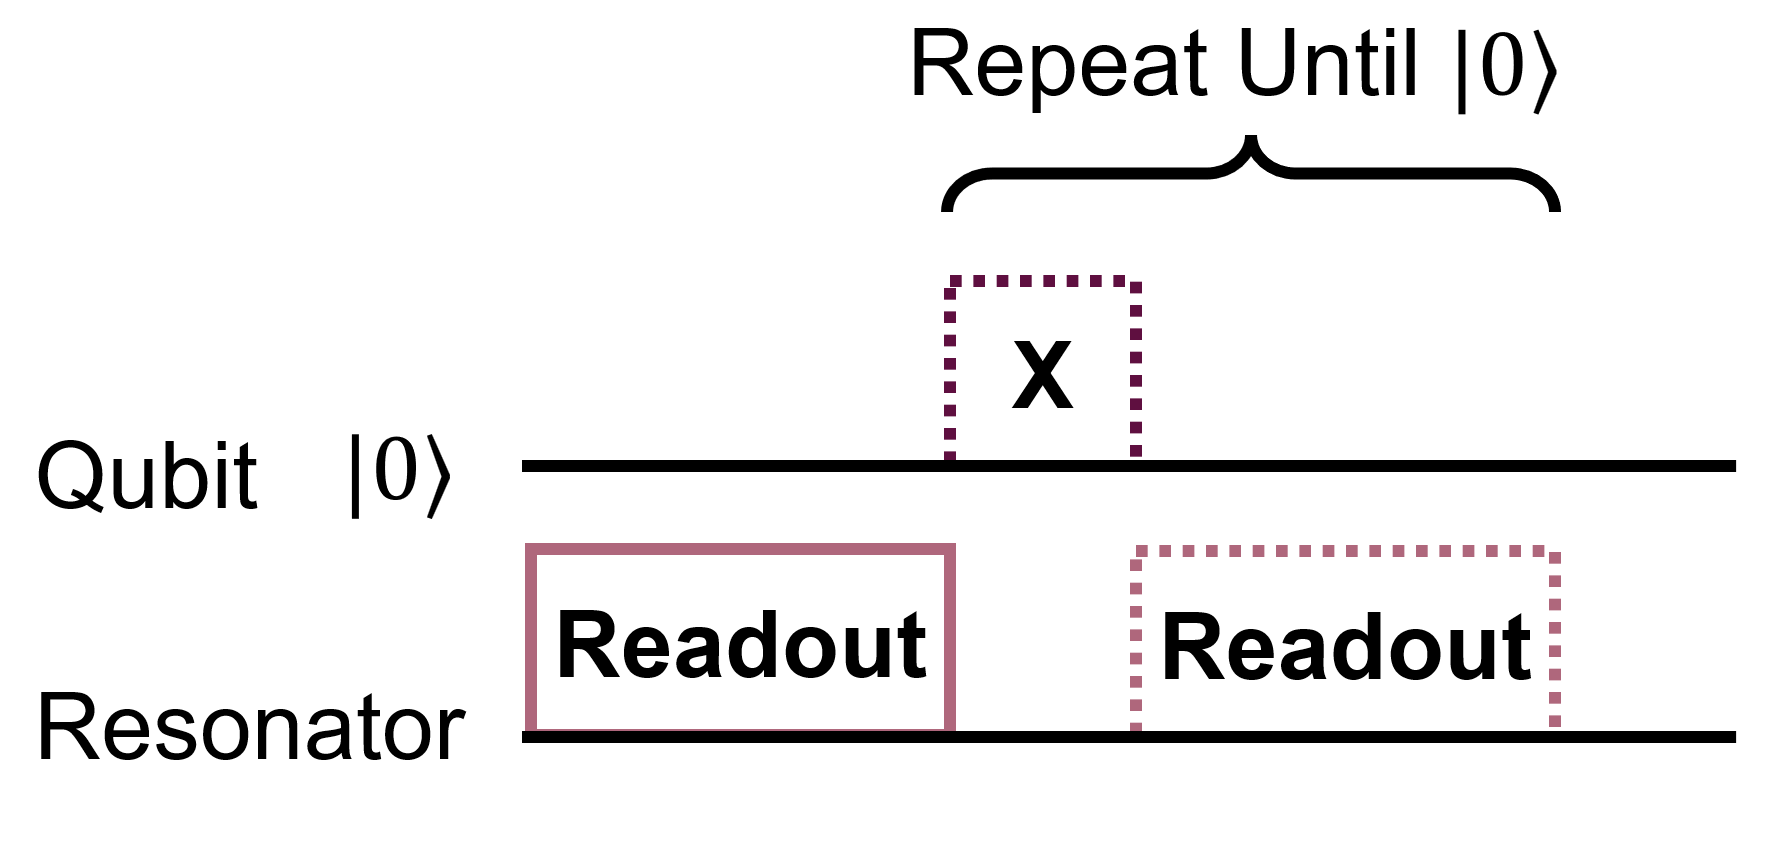
\includegraphics[]{Figs/circuits/active_reset.png}
    \caption{Illustration of the active reset process. A readout is performed, if it measures $\ket{1}$ an $X$-gate and another readout is applied. This is repeat till the readout gives $\ket{0}$.}
    \label{fig:active_reset}
\end{marginfigure}

\subsection{Qubit Decay}
Unwanted changes of the qubit between $\ket{0}\leftrightarrow\ket{1}$ is also a big barrier to reading out the qubit. Since the qubit change state during the readout process, it will be difficult to classify as either $\ket{0}$ or $\ket{1}$ and will often lead to points floating in between in the IQ plots. In table \ref{tab:decay_contribution_estimation}, we see how small reductions in the transition rate increase the readout fidelity. 
\begin{margintable}
\centering
\caption{The outcome of calibrating the qubit with the methods presented in this chapter.}
\vspace{0.3 cm}
\begin{tabular}{lll|c}
\hline
\textbf{Reduction}         &  $\Gamma_1$                  &  $T_1$        & Fidelity (\%)\\ \hline
-10 \%                     &  $0.256 \text{ µs}^{-1}$         &  $3.91$ µs   &  $66 \pm 2$\\
0   \%                     &  $0.232 \text{ µs}^{-1}$         &  $4.30$ µs   &  $65 \pm 2$\\
10  \%                     &  $0.209 \text{ µs}^{-1}$         &  $4.78$ µs   &  $59 \pm 3$\\
25  \%                     &  $0.175 \text{ µs}^{-1}$         &  $5.73$ µs   &  $64 \pm 2$\\
50  \%                     &  $0.116 \text{ µs}^{-1}$         &  $8.60$ µs   &  $70 \pm 2$\\
100 \%                     &  $0$         &  $\infty$                       &  $70 \pm 2$\\
\end{tabular}
\label{tab:decay_contribution_estimation}
\end{margintable}
In section \ref{sec:postselection}, we saw that we can remove most of the measurement errors from this tail by by increasing an overhead and only selecting points which we were the most certain in our classification. However, this will severely impact the ability to run codes and will not be feasible in scenarios like error correcting codes, where a readout is performed on 10s or 100s of qubit in every cycle. 

With a pulse of $600 \text{ ns}$, the contribution from the energy decay during readout seems be less compared to that of efficiency and temperature. Thus, we would probably gain a lot of benefit using the active reset og increasing the pulse length a bit. If we want high-fidelity readout (> 99 \%), we should however find ways to decrease the infidelity contribution from $T_1$ either by improving the device or applying one of the following two adjustmenst.

\paragraph{Shorter Readout Pulse} One way of decreasing the effect of $T_1$ on readout fidelity by making a shorter readout pulse where the qubit can decay. This will however require a higher efficiency since the distance between the two distributions should be at least 3-4 standard deviations to have sub-percent overlap. The distribution we get scale with $1 / \sqrt{\eta t_{\text{readout}}}$ so a higher efficiency and a short pulse could lead to the same results.

\paragraph{Further Excitement} Another method for reducing the impact of qubit decay in readout is by applying a qubit pulse at frequency $f_{12}$ such that we drive transitions $\ket{1}\to\ket{2}$. The $\ket{0}$ will not be affected. And we can choose our readout frequency such that we can draw a decision boundary separating $\ket{0}$ or $\ket{\text{not }0}$ with high fidelity. Since the second excited state $\ket{2}$ primarily relaxes to $\ket{1}$, this will effectively lead to a higher lifetime since $\ket{2}$ and $\ket{1}$ will be classified similarly as $\ket{\text{not} 0}$. Unfortunately, this method can not be combined with active reset, since we only want to apply and x-gate if the qubit is in state $\ket{1}$ and not in this case the indistinguishable $\ket{2}$. This could be solved with good qutrit classification.

% For this reason the further excitement can not be combined with the active reset method presented in the previous subsection.

% Now the readout frequency can be altered to make sure that the Q-function for $\ket{1}$ and $\ket{2}$ are close and easily separable from $\ket{0}$. Since the second excited state $\ket{2}$ first will have to decay to $\ket{1}$ before decaying to $\ket{0}$ \todo{Footnote about fermis golden rule and how this supresses the direct transition} it will increase the readout fidelity. This however comes at the cost of not classifying $\ket{0}$ or $\ket{1}$, but will instead give us $\ket{0}$ or $\ket{\text{not }0}$ since the state could have been in either of the excited states in the measurement. For this reason the further excitement can not be combined with the active reset method presented in the previous subsection.

\subsection{Efficiency}
The efficiency plays a delicate role for reading out. Primarily, it scales the standard deviations of the two gaussian distributions in the IQ plane with a factor of $\sqrt{\eta}$. The overlap between two Gaussians goes rapidly down with smaller widths, and with a separation of only three to four standard deviations, we are below the sub-percent overlap, and we will not see much more performance gain. In \ref{tab:readout_infidelity_contribution_estimation}, we see that a 4 time increase in $\eta$ leads to approximately the same performance gain as by having a perfect efficiency. If we were to be able to go further, we could use this to instead create short pulses capable of the same separation. The following two strategies can be used to combat high infidelity from the efficiency.

% Since it gives a rough estimate to get two Gaussian distributions in the IQ plot., the overlap scales with the amount of standard deviations they are apart. While having a distance at $< 3\sigma$ give an overlap of order a few percent, this drops rapidly after and when the distributions are $5 \sigma$ apart the overlap is negligible especially compared to the contributions from decay and temperature. To see the effect of reducing the inefficiency refer to table \ref{tab:readout_infidelity_contribution_estimation}. 

\begin{margintable}
\centering
\caption{The outcome of calibrating the qubit with the methods presented in this chapter.}
\begin{tabular}{rr|c}
\hline
\textbf{Increase}       &  Efficiency       & Fidelity (\%)\\ \hline
-25 \%                  &  $\;2.64$ \%        &  $65 \pm 2$\\
0   \%                  &  $\;3.30$ \%        &  $65 \pm 2$\\
33  \%                  &  $\;4.40$ \%        &  $68 \pm 2$\\
100  \%                 &  $\;6.60$ \%        &  $68 \pm 2$\\
300  \%                 &  $13.2$ \%          &  $73 \pm 2$\\
max                     &  $100.0$ \%         &  $75 \pm 2$\\
\end{tabular}
\label{tab:readout_infidelity_contribution_estimation}
\end{margintable}

\paragraph{Longer Readout Pulse} The duration of a pulse is a compromise between energy decay and readout efficiency. If the pulse is too short the two distributions can have a big overlap making it hard to classify them, whereas a long pulse allows for energy decay. If we were to have a large $T_1$ and a low efficiency, which we according to the conclusions of last section have in our case. We should probably have a longer readout pulse to find the optimum. 

\paragraph{High Power Readout - } The efficiency helps reduce the overlap of the two distribution by making the distributions narrower. However, another approach is to move them further away from each other. In this thesis, we have been limited by the amount of photon number for numerical reasons. By driving the resonator with a larger amplitude, the two distributions would move further away in the IQ-space. One should however be aware of the increased shift of the qubit frequency and to still be within the critical photon number where the dispersive approximation is valid or venture into a new realm of high power readouts. 


\begin{figure}
    \centering
    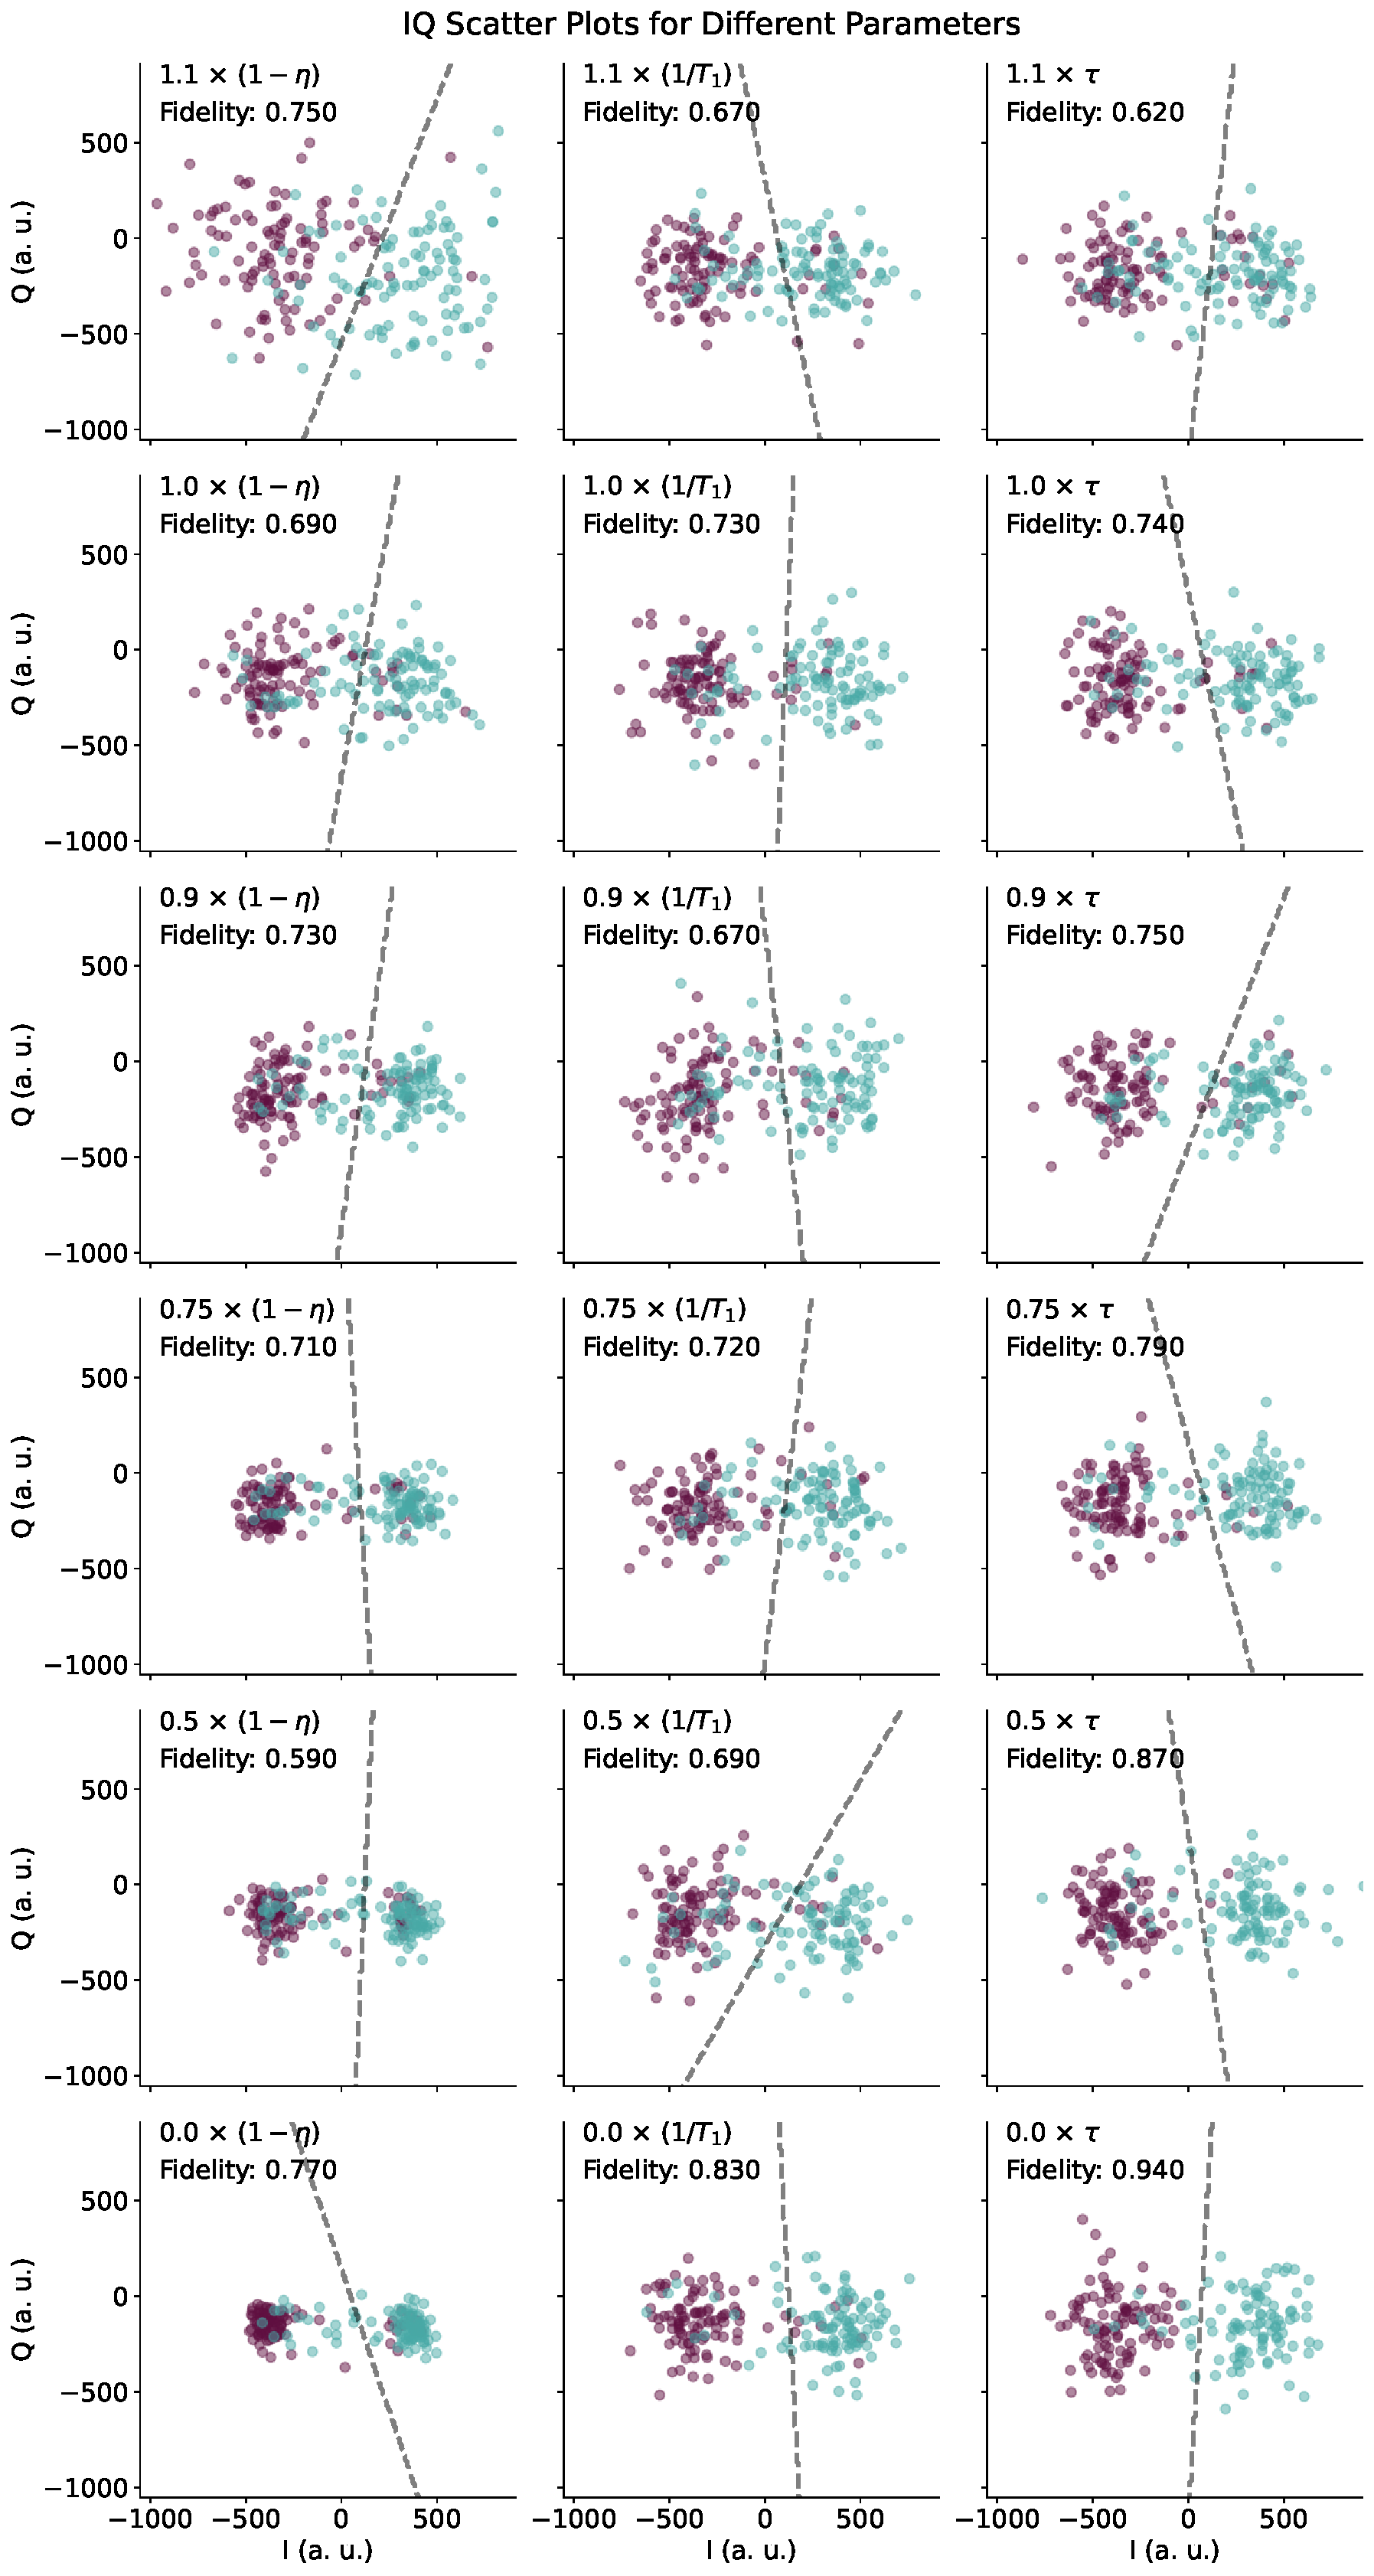
\includegraphics{Simulations/budgets/figures/iq_scatter_budgetting.pdf}
    \caption{The IQ Plots for the models  with different parameters. The seperation line, fidelity and parameter scaling is shown.}
    \label{fig:budgetting_IQ_plots}
\end{figure}
\FloatBarrier

\section{Further Path to Optimization}
In the sections above, we have very much considered a first order optimization, where all except one parameter was kept constant. This gives significant improvements for reductions in temperature, less for increased $\eta$ and marginal increases from better $T_1$. In addition to the improvements from a colder, more coherent and more efficient setup, we also discussed the possibility of "trading" a good performing parameter to improvements in the others. Some of the trade-offs are illustrated in figure \ref{fig:trading_performance}. 

\begin{marginfigure}
    \centering
    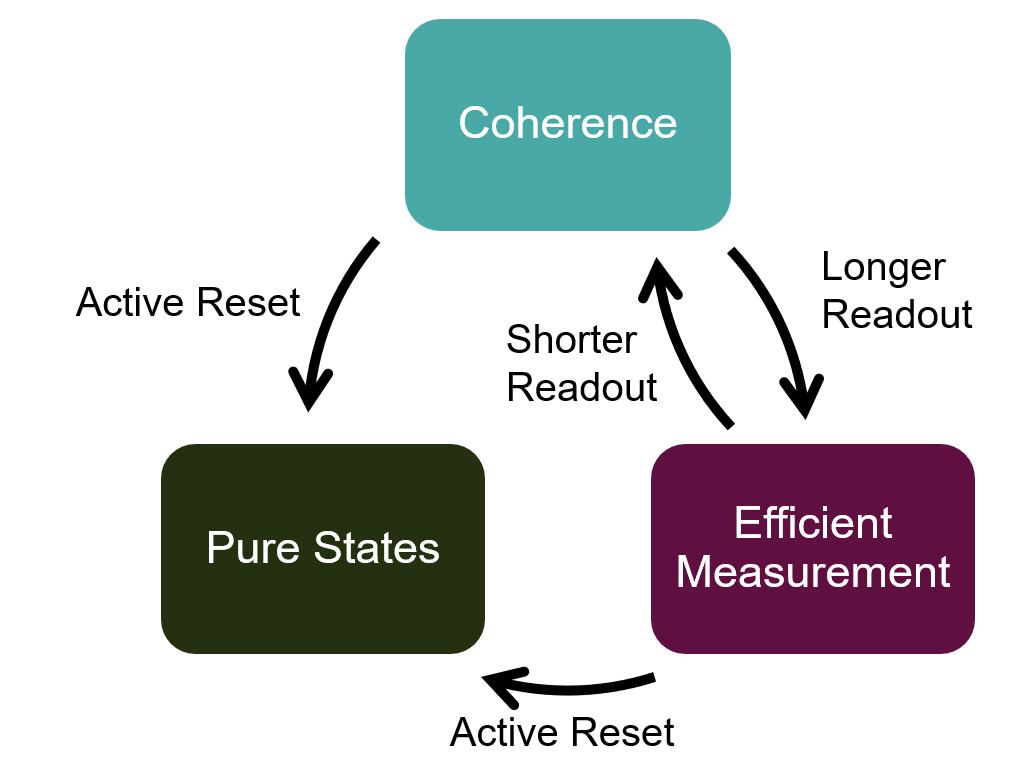
\includegraphics[]{Figs/trading_parameters.png}
    \caption{Illustration of how good coherence, low temperatures or efficient measurement can be used to reduce infidelity contribution from the other sources. }
    \label{fig:trading_performance}
\end{marginfigure}

The biggest factor in our SPAM errors was the temperature providing a mixed state from the beginning. Since the $T_1$ seemed to be less limiting, we would probably benefit from using the active reset method in our approach. Furthermore, we saw that the contribution from efficiency is larger than that of energy decay. Thus, we suspect we could win performance by using a longer pulse. This consideration can be used to do an accumulated demodulation and pick the duration with the lowest overall fidelity.

Since all improvements would lead to an altered readout sequence, the improvement gained by reducing the parameters in the section above are thus not very representative of what would actually happen in the laboratory. To increase performance, a changed parameter would quicly start a search for the optimal readout duration, amplitude and applying the tricks (like active reset) that would help with our setup. In order to use the simulation model we have built up through this thesis, the next steps would be to find ways of simulating these strategies, so they can be applied when we do our forecasts. This will also lead to second order effects like the efficiency classification leaking into the state preparation, if it is done with active reset.

Another challenge is that a stronger pulse would definitely help our readout fidelity. The increased amplitude will force us to use a larger Hilbert space as well. And since the Lindblad Equation and the Stochastic Master Equation both evolve the density matrix, we would effectively get $n^2$ differential equation to solve. Implementing active reset in simulation is also not trivial. In the code-module built for this thesis, the simulation of a trajectory is separate from the analysis and classification from the trajectories. In active reset, we would have to do a simulation, readout analysis and either apply an x-gate or not before simulating again\footnote{And might even have to repeat multiple times if the readout the second time still gives $\ket{1}$}. Since we also need to take into account the cool down of the resonator and the possibility of qubit decay in the meantime, this would ultimately mean a 3-10 times increase  (at best)  of simulation time and would require a much more flexible simulation module.